
\section{Data Analysis with \texttt{R}}

Data from Table 1.1 of the textbook

Table 1.1 Random and systematic errors

\begin{tabular}{|c|ccccc|l|}
	\hline
	% after \\: \hline or \cline{col1-col2} \cline{col3-col4} ...
	Student & Results  & (ml) &  &  &  &Comment \\ \hline
	A & 10.08 & 10.11 &10.09 &10.10&10.12 & Precise, unbiased\\ \hline
	B & 9.88 &10.14& 10.02 &9.80& 10.21& Imprecise unbiased\\ \hline
	C & 10.19 &9.79& 9.69 &10.05& 9.78 & Imprecise, biased\\ \hline
	D & 10.04 &9.98 &10.02 &9.97 &10.04 & Precise, unbiased \\
	\hline
\end{tabular}
\bigskip

This is also given in the text file Table$1-1$.txt, the contents of which is given below:
\begin{center}
	\line(1,0){250}
\end{center}
\begin{verbatim}
A 10.08 10.11 10.09 10.10
B 9.88 10.14 10.02 9.80
C 10.19 9.79 9.69 10.05
D 10.04 9.98 10.02 9.97
\end{verbatim}
\begin{center}
	\line(1,0){250}
\end{center}

Reading data from a file to \texttt{R}:
\begin{center}
	\line(1,0){250}
\end{center}
\begin{verbatim}
#Reading the data from
Titra=read.table("Table1-1.txt", row.names = 1)
Titra
# V2 V3 V4 V5
#A 10.08 10.11 10.09 10.10
#B 9.88 10.14 10.02 9.80
#C 10.19 9.79 9.69 10.05
#D 10.04 9.98 10.02 9.97
#Listing the first row
Titra[1,]
#and the fourth column
Titra[,4]
\end{verbatim}
\begin{center}
	\line(1,0){250}
\end{center}

\textbf{Means and standard deviations}\\

Find the mean and standard deviation of A's results.

\begin{center}
	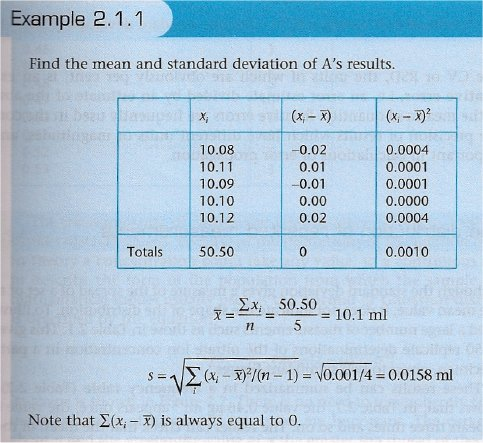
\includegraphics[scale=0.6]{Image8}
\end{center}


\textbf{Means and standard deviations much faster and better}
\begin{center}
	\line(1,0){250}
\end{center}
\begin{verbatim}
#Comuting means
rowMeans(Titra)
# A B C D
#10.0950 9.9600 9.9300 10.0025
#and standard deviation
apply(Titra,1,sd)
# A B C D
#0.01290994 0.15055453 0.23036203 0.03304038
\end{verbatim}
\begin{center}
	\line(1,0){250}
\end{center}
\newpage
\textbf{Nitrate ion concentration from Table 2.1}\\
Table 2.1 Results of 50 determinations of nitrate ion concentration, in $\mu$g $ml^{-1}$ (Also in the file Table $2-1$.txt.) \\
\begin{tabular}{|c|c|c|c|c|c|c|c|c|c|}
	\hline
	0.51 &0.51 &0.51 &0.50 &0.51 &0.49 &0.52 &0.53 &0.50 &0.47\\
	0.51 &0.52 &0.53 &0.48 &0.49 &0.50 &0.52 &0.49 &0.49 &0.50\\
	0.49 &0.48 &0.46 &0.49 &0.49 &0.48 &0.49 &0.49 &0.51 &0.47\\
	0.51 &0.51 &0.51 &0.48 &0.50 &0.47 &0.50 &0.51 &0.49 &0.48\\
	0.51 &0.50 &0.50 &0.53 &0.52 &0.51 &0.50 &0.50 &0.51 &0.51\\
	\hline
\end{tabular}\\ \bigskip

\begin{center}
	\line(1,0){250}
\end{center}
\begin{verbatim}
0.51 0.51 0.51 0.50 0.51 0.49 0.52 0.53 0.50 0.47
0.51 0.52 0.53 0.48 0.49 0.50 0.52 0.49 0.49 0.50
0.49 0.48 0.46 0.49 0.49 0.48 0.49 0.49 0.51 0.47
0.51 0.51 0.51 0.48 0.50 0.47 0.50 0.51 0.49 0.48
0.51 0.50 0.50 0.53 0.52 0.51 0.50 0.50 0.51 0.51
\end{verbatim}
\begin{center}
	\line(1,0){250}
\end{center}
Compute the mean concentration, and the standard deviation:
\begin{center}
	\line(1,0){250}
\end{center}
\begin{verbatim}
#Getting data in a vector
x=scan('Table2_1.txt')
mean(x)
#[1] 0.4998
sd(x)
#[1] 0.01647385
\end{verbatim}
\begin{center}
	\line(1,0){250}
\end{center}
\newpage


\section{Data Analysis with \texttt{R}}

Data from Table 1.1 of the textbook

Table 1.1 Random and systematic errors

\begin{tabular}{|c|ccccc|l|}
	\hline
	% after \\: \hline or \cline{col1-col2} \cline{col3-col4} ...
	Student & Results  & (ml) &  &  &  &Comment \\ \hline
	A & 10.08 & 10.11 &10.09 &10.10&10.12 & Precise, unbiased\\ \hline
	B & 9.88 &10.14& 10.02 &9.80& 10.21& Imprecise unbiased\\ \hline
	C & 10.19 &9.79& 9.69 &10.05& 9.78 & Imprecise, biased\\ \hline
	D & 10.04 &9.98 &10.02 &9.97 &10.04 & Precise, unbiased \\
	\hline
\end{tabular}
\bigskip

This is also given in the text file Table$1-1$.txt, the contents of which is given below:
\begin{center}
	\line(1,0){250}
\end{center}
\begin{verbatim}
A 10.08 10.11 10.09 10.10
B 9.88 10.14 10.02 9.80
C 10.19 9.79 9.69 10.05
D 10.04 9.98 10.02 9.97
\end{verbatim}
\begin{center}
	\line(1,0){250}
\end{center}

Reading data from a file to \texttt{R}:
\begin{center}
	\line(1,0){250}
\end{center}
\begin{verbatim}
#Reading the data from
Titra=read.table("Table1-1.txt", row.names = 1)
Titra
# V2 V3 V4 V5
#A 10.08 10.11 10.09 10.10
#B 9.88 10.14 10.02 9.80
#C 10.19 9.79 9.69 10.05
#D 10.04 9.98 10.02 9.97
#Listing the first row
Titra[1,]
#and the fourth column
Titra[,4]
\end{verbatim}
\begin{center}
	\line(1,0){250}
\end{center}

\textbf{Means and standard deviations}\\

Find the mean and standard deviation of A's results.

\begin{center}
	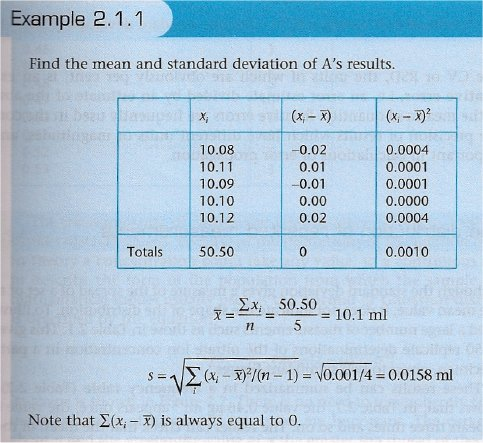
\includegraphics[scale=0.6]{Image8}
\end{center}


\textbf{Means and standard deviations much faster and better}
\begin{center}
	\line(1,0){250}
\end{center}
\begin{verbatim}
#Comuting means
rowMeans(Titra)
# A B C D
#10.0950 9.9600 9.9300 10.0025
#and standard deviation
apply(Titra,1,sd)
# A B C D
#0.01290994 0.15055453 0.23036203 0.03304038
\end{verbatim}
\begin{center}
	\line(1,0){250}
\end{center}
\newpage
\textbf{Nitrate ion concentration from Table 2.1}\\
Table 2.1 Results of 50 determinations of nitrate ion concentration, in $\mu$g $ml^{-1}$ (Also in the file Table $2-1$.txt.) \\
\begin{tabular}{|c|c|c|c|c|c|c|c|c|c|}
	\hline
	0.51 &0.51 &0.51 &0.50 &0.51 &0.49 &0.52 &0.53 &0.50 &0.47\\
	0.51 &0.52 &0.53 &0.48 &0.49 &0.50 &0.52 &0.49 &0.49 &0.50\\
	0.49 &0.48 &0.46 &0.49 &0.49 &0.48 &0.49 &0.49 &0.51 &0.47\\
	0.51 &0.51 &0.51 &0.48 &0.50 &0.47 &0.50 &0.51 &0.49 &0.48\\
	0.51 &0.50 &0.50 &0.53 &0.52 &0.51 &0.50 &0.50 &0.51 &0.51\\
	\hline
\end{tabular}\\ \bigskip

\begin{center}
	\line(1,0){250}
\end{center}
\begin{verbatim}
0.51 0.51 0.51 0.50 0.51 0.49 0.52 0.53 0.50 0.47
0.51 0.52 0.53 0.48 0.49 0.50 0.52 0.49 0.49 0.50
0.49 0.48 0.46 0.49 0.49 0.48 0.49 0.49 0.51 0.47
0.51 0.51 0.51 0.48 0.50 0.47 0.50 0.51 0.49 0.48
0.51 0.50 0.50 0.53 0.52 0.51 0.50 0.50 0.51 0.51
\end{verbatim}
\begin{center}
	\line(1,0){250}
\end{center}
Compute the mean concentration, and the standard deviation:
\begin{center}
	\line(1,0){250}
\end{center}
\begin{verbatim}
#Getting data in a vector
x=scan('Table2_1.txt')
mean(x)
#[1] 0.4998
sd(x)
#[1] 0.01647385
\end{verbatim}
\begin{center}
	\line(1,0){250}
\end{center}
\newpage